\label{sec:ui}

\subsection{\Tool IDE Plugin Features}
We have implemented \Tool as an IDE plugin for RubyMine \cite{RubyMine}, a popular IDE
for Ruby on Rails. A screenshot of \Tool is shown in 
Figure~\ref{fig:pw}. By pressing the ``PowerStation'' button 
at the top of RubyMine, users can choose an analysis scope, 
``Whole Application'' or ``Single Action,''
and launch \Tool analysis accordingly. 
%``Whole Application'' starts \Tool by performing static analysis on the loaded application code. ``Single Action'' allows users to choose a single action and performs analysis on its source code. 
Our website includes a tutorial~\cite{powerstation}.

\textbf{Issues list.} The right panel, as highlighted in Figure \ref{fig:pw}, lists all the
inefficiencies detected by \Tool, each represented by a button displaying the file where
the inefficiency is located. 
By default, all the inefficiencies found in the project are listed. %\shan{right?}.
Users can also choose to display inefficiencies of a particularly type as shown in Figure \ref{fig:pw}---loop invariant queries (LI), dead store queries (DS), unused data retrieval queries (RD), 
common sub-expression queries (CS), API misuses (IA), and inefficient rendering (IR).

\textbf{Issues highlight.} 
Clicking the file button in the issue list will navigate users 
to the corresponding file in the editor, with the inefficient code 
highlighted. Hovering the cursor over the highlighted code will display the reason for highlighting, as shown in Figure~\ref{fig:pw}.
%, it shows that under the dead-store query anti-pattern category, there is one file named \textit{blogs\_controller.rb}, and the left editor highlights line 33, and line 34 which involves the dead store queries. 

\textbf{Issue fix.} Clicking the ``fix'' button next to each issue in the issue list will 
pop up window asking the user whether she wants \Tool to fix the issue. If so, \Tool will synthesize a fix as discussed in 
Section~\ref{sec:impl}, and display the fixed code in the editor panel. 
At that point, the original ``fix'' button becomes an ``undo'' button, allowing users to revert the fix if needed.

\begin{figure}
\centering
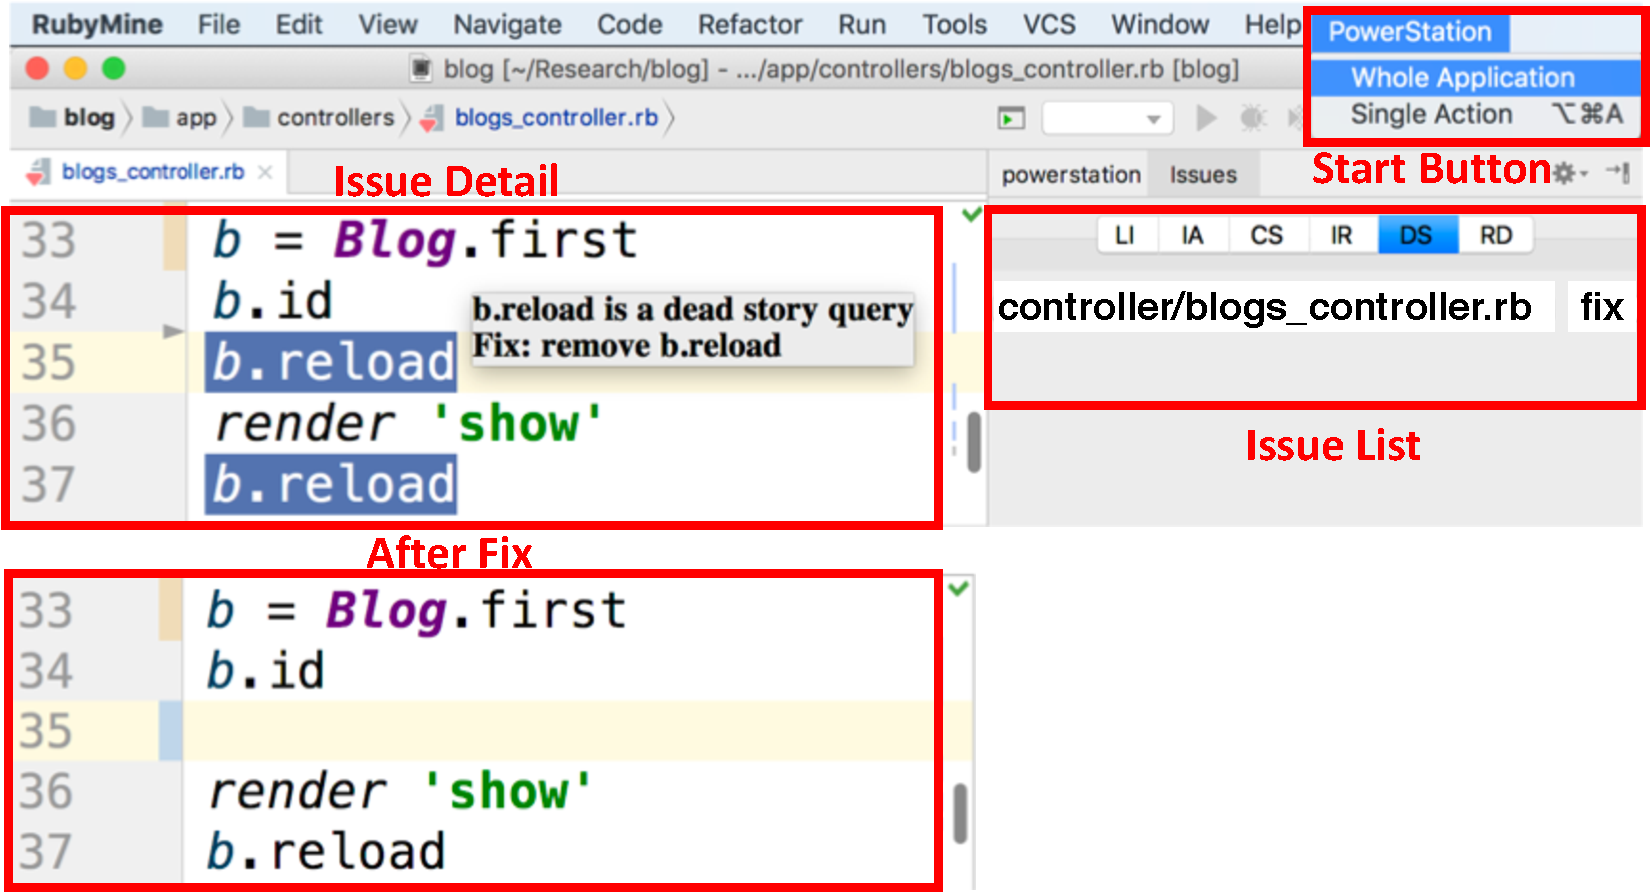
\includegraphics[width=0.9\columnwidth]{figs/after.pdf}
\vspace{-0.1in}
\caption{Screenshots of \Tool IDE Plugin}
\label{fig:pw}

\vspace{-0.25in}
\end{figure}

% \begin{figure}
% \centering
% 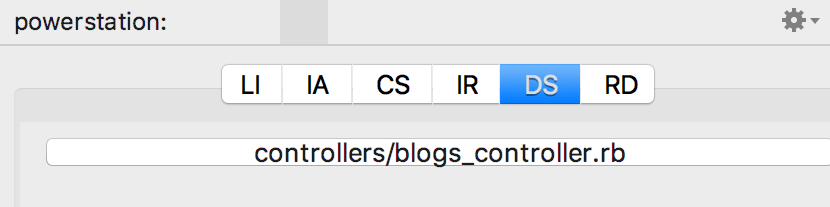
\includegraphics[width=\columnwidth]{figs/issue-list}
% \vspace{-0.1in}
% \caption{Issue list of PowerStation%\shan{this figure is really wasting space. we should have such snapshots but need to contain much more information\ than this. maybe multiple shots are better?}
% }

% \label{fig:issue-list}
% \end{figure}
\begin{comment}

\begin{figure}[t!]
%\centering
%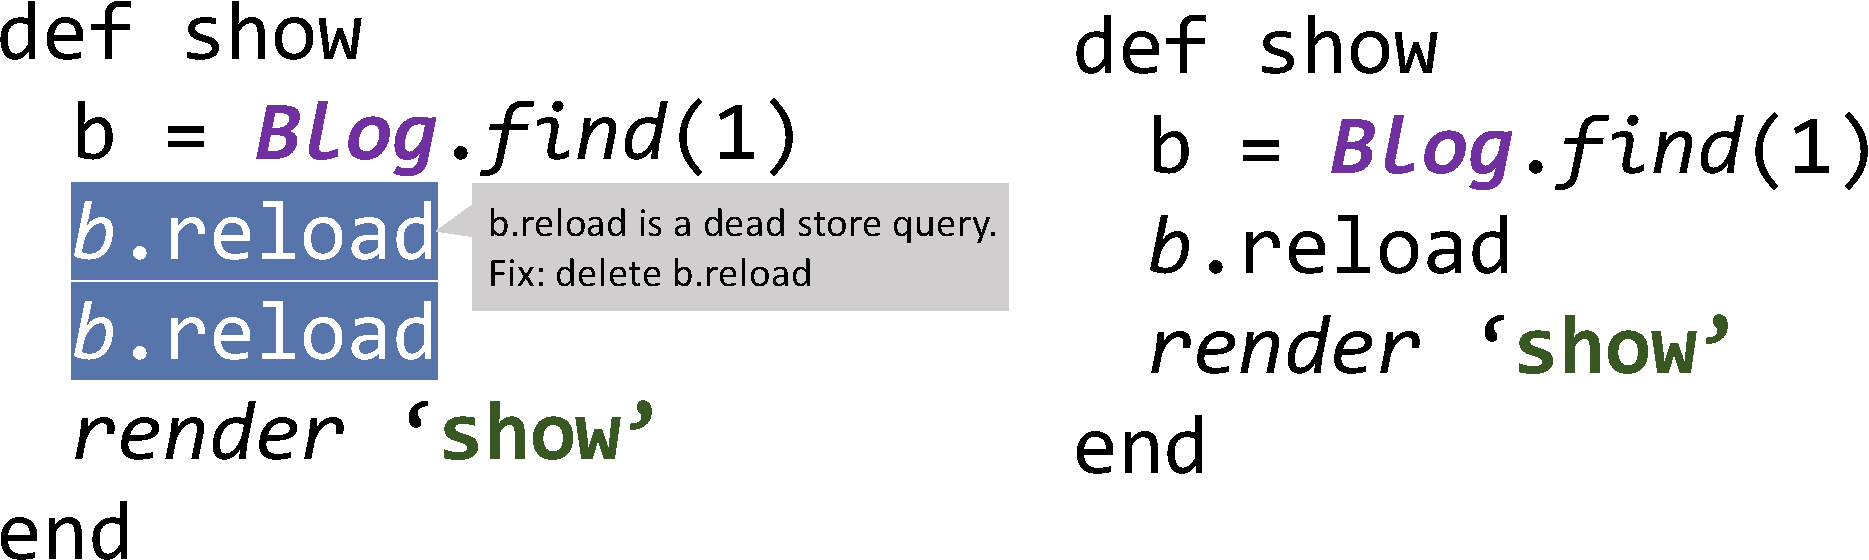
\includegraphics[width=\columnwidth]{figs/issue-detail}
\begin{subfigure}[t]{0.5\textwidth}
        \centering
        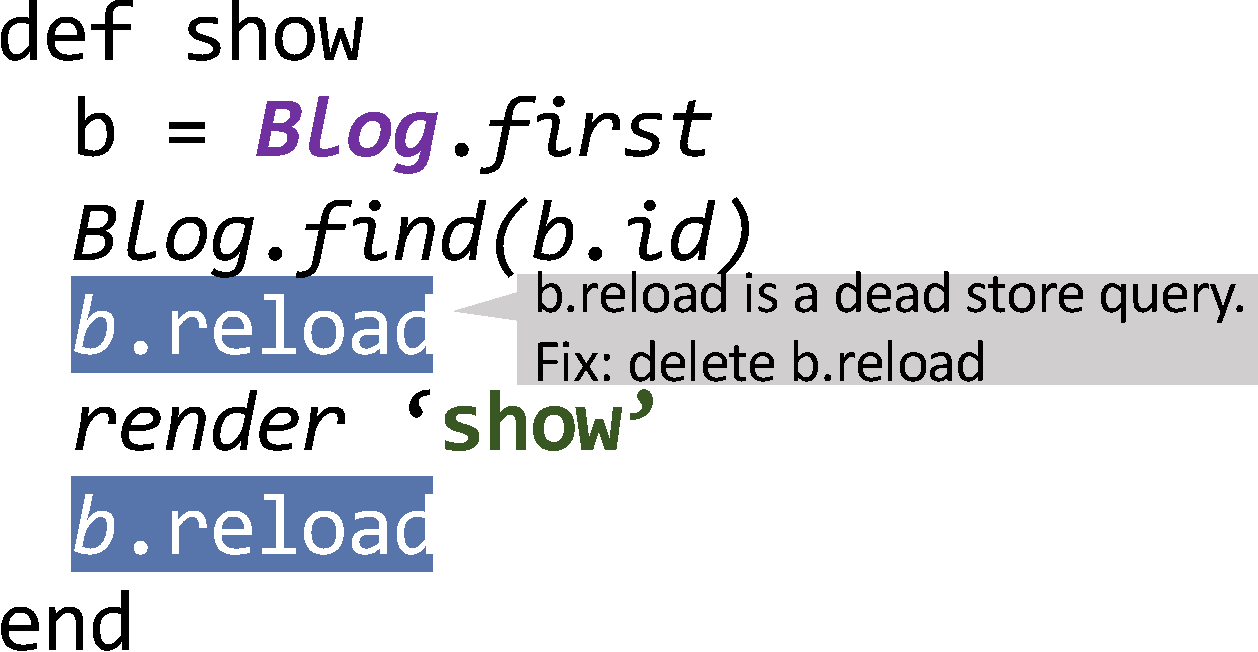
\includegraphics[width=0.45\columnwidth]{figs/before.pdf}
        \caption{Before fix}
        \label{fig:bfix}
 \end{subfigure}%
 \begin{subfigure}[t]{0.5\textwidth}
        \centering
        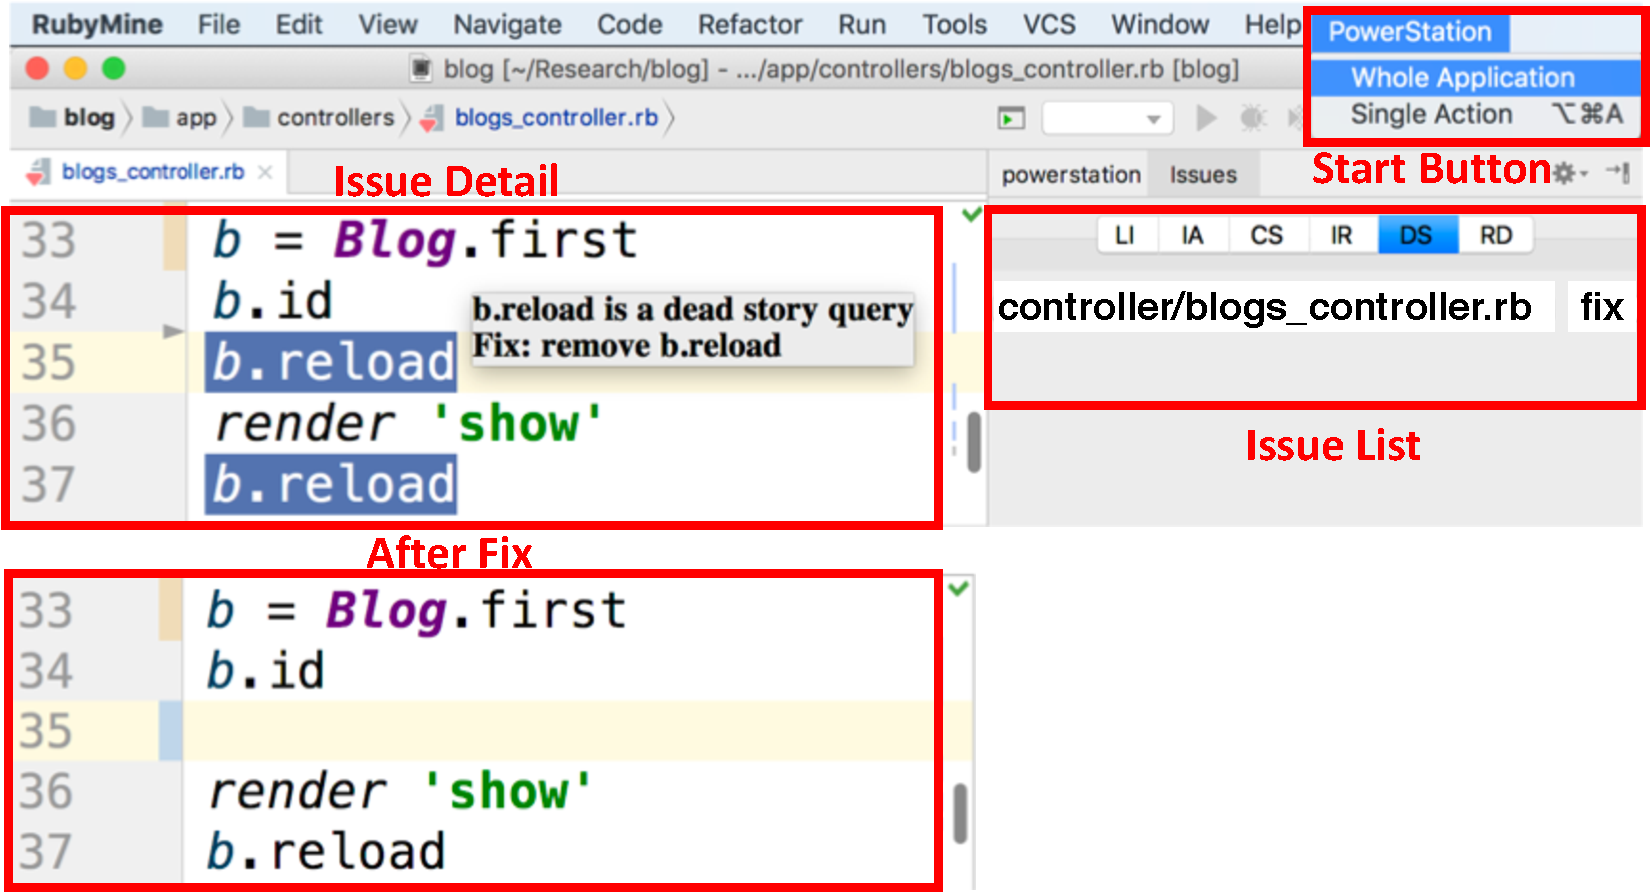
\includegraphics[width=0.45\columnwidth]{figs/after.pdf}
        \caption{After fix}
        \label{fig:afix}
 \end{subfigure}%
\vspace{-0.1in}
\caption{Issue details in Editor \shan{Very strange figures. 1. The code on the left is 
different from the code in Figure 6; 2. It is unclear what is the relationship between
the left side and the right side; } }
\label{fig:ide}
\end{figure}

\end{comment}

\vspace{-2mm}
\subsection{Implementation}

We used the APIs provided by the
IntelliJ Platform like {\tt ToolWindow} and
%~\cite{toolwindow} and 
{\tt JBTabbedPane}
%~\cite{guidesigner} 
to create the \Tool issues list.

Highlighting the selected inefficiency is straight-forward using
the IntelliJ API {\tt HighlighterLayer}, given file name and line number provided by \Tool static analysis.

For every anti-pattern, \Tool prepares a string template that explains the inefficiency and the fix strategy,
such as ``* is a dead store query. Fix: delete *.'' for a dead-store query (Figure \ref{fig:pw}). This string
is instantiated with program variables and expressions output from \Tool static analysis, and displayed using
the IntelliJ API {\tt FileDocumentManager}.

Finally, IntelliJ API {\tt FileEditorManager}, {\tt TextRange}, and {\tt Document} are used to insert, replace, and delete source code
in the editor panel. 
%Table~\ref{tab:fixop} shows the fix operation needed for different anti-patterns.

\iffalse
\begin{table}[H]
    \centering
    \begin{tabular}{c|c}
    \toprule
         API Misuse  & replacement \\ 
        Loop Invariant Query &  insertion and replacement\\ Dead-store Query  &  deletion\\ 
        Unnecessary Data Retrieval  & deletion or replacement\\
         Inefficient Rendering &insertion and replacement \\
         \bottomrule
    \end{tabular}
    \caption{Fix Operation}
    \label{tab:fixop}
\end{table}
\fi
%The IntelliJ Platform provides all of the infrastructure which IDEs need to provide rich language tooling support. It has a component driven, cross platform JVM based application host with a high level user interface toolkit. By using it we are able to create tool windows which will be used to show the performance issue list, and we can create popup menus  used to show the details of the performance issues and the fix suggestions. Moreover, it also includes a full text editor, and provides abstract implementations of syntax highlighting, code folding, code completion, which we use to highlight the code involving in the anti-patterns. Also, Program Structure Interface (PSI) enables  quick navigating to files which allows us to open the specified files which contain the performance issues source code. Also, code inspections and code rewriting provided by PSI gives us opportunity to do quick fixes or refactorings.

%IntelliJ is a platform for building multi-language IDE's and plugins, and includes components such as UI elements, a text editor, frameworks for code manipulation, including code navigation and inspection, and plugin development APIs.  It also supports code execution and debugging.


%The main APIs that were used from the Intellij Platform in implementing Powerstation include the IntelliJ plugin development API and Java's Swing and AWT APIs.  The IntelliJ plugin development API was used for operations that use the source code of the inputted project or change properties of the IDE.  In particular, it was used to read and write source code (e.g. string-matching and replacing inefficient API uses), navigate to specific files which contain the source code for performance issues, highlight code, and embed the Powerstation plugin into the IDE by adding an IDE menu option for it. Java's Swing and AWT APIs were used to create visual components of Powerstation's user interface (UI).  In particular, they were used to create a side window giving the user a choice of the issue they want to fix, a tool window that displays a list of performance issues, a checkbox that displays the performance issues by category, file name, and line number, and a pop-up menu with fix suggestions.

